%%%% Header %%%%%%%%%%%%%%%%%%%%%%%%%%%%%%%%%%%%%%%%%%%%%%%%%%%%%%%%%%%%

\documentclass[
  10pt, twoside
]{book}

%%%% Packages %%%%%%%%%%%%%%%%%%%%%%%%%%%%%%%%%%%%%%%%%%%%%%%%%%%%%%%%%%

\usepackage[utf8]{inputenc} % .tex-file text encoding
\usepackage[T1]{fontenc}    % vector fonts and special chars in output
\usepackage{newtxtext, newtxmath} % Times Roman font family

\usepackage{pdfpages} % include external pdfs

%%%% Meta data %%%%%%%%%%%%%%%%%%%%%%%%%%%%%%%%%%%%%%%%%%%%%%%%%%%%%%%%%

\usepackage[
  pdfauthor   ={Jonas Schöley},
  pdftitle    ={The dynamics of ontogenescence},
  pdfsubject  ={},
  pdfkeywords ={},
  pdfproducer =Latex,
  pdfcreator  =pdflatex
]{hyperref}

%%%% Options %%%%%%%%%%%%%%%%%%%%%%%%%%%%%%%%%%%%%%%%%%%%%%%%%%%%%%%%%%%


\usepackage{geometry}
\geometry{
  paperheight = 24cm,
  paperwidth  = 17cm,
  top         = 2.54cm,
  bottom      = 2.54cm,
  inner       = 2cm,
  outer       = 2.54cm,
  footskip    = 11mm,
  headheight  = 1cm,
  headsep     = 0.75cm,
  showframe   = false
}

\setlength{\parskip}{0.5ex}
\setlength{\parindent}{0cm}

%%%% Titlepage %%%%%%%%%%%%%%%%%%%%%%%%%%%%%%%%%%%%%%%%%%%%%%%%%%%%%%%%%

\begin{document}

\begin{titlepage}
\begin{center}
{\huge\bfseries The dynamics of ontogenescence: \\ Modelling age trajectories of \\ feto-infant mortality\\}
% ----------------------------------------------------------------
  \vspace{1.5cm}
{\Large\bfseries Jonas Schöley}\\[5pt]
% ----------------------------------------------------------------
  \vspace{2cm}
{Thesis  submitted to} \\[5pt]
\emph{{University of Southern Denmark}}\\[2cm]
{in partial fulfillment for the award of the degree
  of} \\[2cm]
\textsc{\Large{{Doctor of Philosophy}}} \\[5pt]
\vfill
{Faculty of Health Sciences}\\[5pt]
{Department of Public Health}\\[5pt]
{Interdisciplinary Centre on Population Dynamics}\\
\vfill
{Odense, Denmark}\\[5pt]
{June 2020}
\end{center}
\end{titlepage}

\pagenumbering{gobble}

%%%% Supervisors %%%%%%%%%%%%%%%%%%%%%%%%%%%%%%%%%%%%%%%%%%%%%%%%%%%%%%%

{\noindent\footnotesize
  \textbf{\Large Academic Advisors}
  \vspace{0.5cm}\\
  Professor \textbf{James W. Vaupel}, Ph.D.\\
  Interdisciplinary Centre on Population Dynamics\\
  University of Southern Denmark
  \vspace{0.4cm}\\
  Associate Professor \textbf{James Oeppen}, M.A.\\
  Interdisciplinary Centre on Population Dynamics\\
  University of Southern Denmark
  \vspace{0.4cm}\\
  Professor \textbf{Rune Lindahl-Jacobsen}, Ph.D.\\
  Interdisciplinary Centre on Population Dynamics\\
  University of Southern Denmark
}
\vfill
{\noindent\footnotesize
  \textbf{\Large Assessment Committee}
  \vspace{0.5cm}\\
  Professor \textbf{Michel Guillot}, Ph.D.\\
  Department of Sociology \& Population Studies Center\\
  University of Pennsylvania
  \vspace{0.4cm}\\
  Professor \textbf{Laust Hvas Mortensen}, Ph.D.\\
  Department of Public Health\\
  University of Copenhagen
  \vspace{0.4cm}\\
  Professor \textbf{Jesper Lier Boldsen}, Ph.D.\\
  Institute of Forensic Medicine\\
  University of Southern Denmark
}

\clearpage

%%%% Dedication %%%%%%%%%%%%%%%%%%%%%%%%%%%%%%%%%%%%%%%%%%%%%%%%%%%%%%%%

{
\vspace*{\stretch{1}}
\itshape
\raggedleft
Dedicated to Hans Richter
\par
\vspace{\stretch{3}}
}
   
\clearpage


%%%% Table of contents %%%%%%%%%%%%%%%%%%%%%%%%%%%%%%%%%%%%%%%%%%%%%%%%%

\tableofcontents

\clearpage

%%%% Preface %%%%%%%%%%%%%%%%%%%%%%%%%%%%%%%%%%%%%%%%%%%%%%%%%%%%%%%%%%%

\pagenumbering{roman}
\pagestyle{plain}

\section*{Preface}
\addcontentsline{toc}{section}{Preface}

My maternal grandfather was the optometrist in a small village close to what used to be the international border separating east and west Germany. Long retired, his home-office still looks very much like I remember it from my childhood days. Amongst his library of books, one can find old medical scales, a human skull, geological samples, ancient arrow tips found in the field, a star chart, a lunar globe, a microscope, and other instruments which would not look out of place in a reimagination of Victorian-era science. His scientific ambitions, however, remained unfulfilled. In the ``German Democratic Republic'' a person's aptitude for science was not the most important requirement for the \emph{permission} to engage in doctoral studies. Opa, your ongoing curiosity has been an inspiration to me. I dedicate this thesis to you -- but not without thanking Grandmother as well -- Oma, wasn't it you who paid the rent while Opa was studying for his diploma?

The academic ambitions of one person tend to affect the whole family. I've finished this thesis during the Corona pandemic, at home with my wife Anja and my son Linus. Anja, not only did you allow me to write under rather unusual circumstances, but you've also given me perspective whenever I needed it, i.e., constantly; and so did you Linus: you've grown faster than my thesis and having you was the best decision I've ever made. Also, going through an elaborate good-night ritual with you Linus was a welcome distraction during the final writing stage.

Jim, you've recruited me into the Ph.D. program, set me up with a big research question, and gave me the freedom not only to approach the topic on my own but also to do so while being with my family. For all that, I thank you. The range of research and teaching activities I was allowed to engage in have given me the experience I would have never gained under a more restrictive supervisor.
  
I thank my co-supervisors Jim Oeppen and Rune Lindahl-Jacobsen for their support and for always promptly commenting on the drafts I sent them.

I thank Roland Rau, who taught me the joy of programming; Frans Willekens and Trifon Missov, who prompted me to start my Ph.D. journey; Steffi, who was a fantastic room-mate; Catalina, with whom I've had such honest conversations; Marius, who made everything look so easy; Rita, who selflessly helped me out; Anthony, who more than once shared his wisdom with me; Tim, who gave me plenty opportunities to build a research profile; Ilya, with whom I engaged in incredibly productive procrastination; my ThinkPad, which has been a reliable tool for the last five years; all my friends from EDSD, with whom I spent an incredible time in Warsaw; and my parents, who never questioned the path I've taken.

\clearpage

%%%% English summary %%%%%%%%%%%%%%%%%%%%%%%%%%%%%%%%%%%%%%%%%%%%%%%%%%%

\section*{English summary}
\addcontentsline{toc}{section}{English summary}

Even before our lives begin, we are on an escape trajectory from death. It has been estimated that out of 100 conceptions around 66 do not survive until the clinical recognition of pregnancy. The risk of in-utero death then declines until the third trimester, yet for some, the struggle of labor acts as a barrier of entry to life with most infant deaths in the U.S. nowadays occurring within the first seven days following birth. From there on, survival prospects improve continuously until the onset of adolescence.

The pattern of declining death rates before maturity has been observed all across nature, and, as the mirror image of the senescent increase in mortality later in life, the phenomenon has been coined \emph{ontogenescence}.

What drives ontogenescence? Despite its potentially deep evolutionary roots, there are three more immediate explanations: 1) \emph{acquired robustness} due to continued growth and development of the fetus and infant, 2) \emph{mortality selection} leading to declining death rates on the cohort level as those with the highest individual risk of death tend to die early, and 3) \emph{transitional timing}, meaning the clustering of risky transitions early in life.

This thesis aims to separate the three explanations by defining measurements for each and applying them to detailed data on fetal and infant survival for the United States. I contribute to the demographic study of age trajectories of mortality by proposing and validating a general family of hazard models for infant mortality, connecting this family to frailty and shock theory, explicitly testing the mortality selection hypothesis by considering the observed distribution of risk among neonates and presenting the phenomenon of the ``birth hump'' in the context of mortality over the age of gestation.

In the first paper, it is shown that many of the parametric models commonly used to describe the age trajectory of infant mortality are part of a class of probability distributions I call the power-exponential hazard family. I demonstrate that the family can conveniently be fitted within the framework of Generalized Linear Models and provide evidence that the trajectory of infant mortality in the United States, measured over days of age, is extremely well captured by said hazard. Interpreted as a ``frailty model'', the power-exponential hazard has a natural connection to the hypothesis of mortality selection, which I explore, while interpreted as the description of a ``thinned Poisson process'', the hazard points towards the transitional timing hypothesis. In both cases, the component of acquired robustness is reflected in an individual level exponentially declining hazard with a ``rate of ontogenescence'' around one percent per day of age.

In paper two, the mortality selection hypothesis is put to the test by explicitly considering the level and shape of neonatal hazard trajectories across 252 mutually exclusive population strata. Surprisingly, despite mortality levels among a population of newborns spanning five orders of magnitude, I find no evidence for the age-trajectory of infant mortality being shaped by selective dropout. The reason for that lies within a remarkable mortality convergence of extremely frail newborns towards the population average: Hazard trajectories in the days following birth are strikingly non-proportional as survival prospects among even the most vulnerable newborns improve drastically once the first day of life has passed.

Having cast doubt on the selection hypothesis, I consider the transitional shock of birth in greater detail. A natural timescale for studying the effect of labor on the survival of a cohort is the age of gestation measured in weeks since the last menses of the mother. Unlike chronological age, the gestational time scale allows for existence before infancy, thereby making it possible to study birth as a transition. On the aggregate level, this transition appears as a ``hump'' in an otherwise exponentially declining hazard of death for a cohort of fetuses as we follow them on their way into life. I study this gestational age pattern across multiple populations with a particular focus on describing the phenomenon of the ``birth hump''.

\clearpage

%%%% Dansk resumé %%%%%%%%%%%%%%%%%%%%%%%%%%%%%%%%%%%%%%%%%%%%%%%%%%%%%%

\section*{Dansk resumé}
\addcontentsline{toc}{section}{Dansk resumé}

Allerede inden vores liv begynder, befinder vi os i en flugt fra døden. Det er blevet estimeret, at 66 ud af 100 undfangelser ikke når til den kliniske anerkendelse af graviditet. Risikoen for død i livmoderen falder derefter indtil tredje trimester, men for nogle fungerer arbejdskampen som en barriere for adgangen til livet med de fleste spædbørnsdødsfald i USA i dag, der forekommer inden for de første 7 dage efter fødslen. Derfra forbedres udsigterne til at overleve kontinuerligt indtil ungdomsårenes begyndelse.

Mønsteret med faldende dødsrater inden modenhed er blevet observeret overalt i naturen, og som et spejlbillede af den aldersbetingede stigning i dødelighed senere i livet, er fænomenet blevet betegnet \emph{ontogenescence}.

Hvad driver ontogenescence? På trods af de potentielt dybe evolutionære rødder er der yderligere tre mere umiddelbare forklaringer: 1) \emph{acquired robustness} på grund af fortsat vækst og udvikling af fosteret og spædbarnet, 2) \emph{mortality selection} der fører til faldende dødsrater på kohorte-niveau, da dem med den højeste individuelle døds-risiko har tendens til at dø tidligere, og 3) \emph{transitional timing} hvilket angiver klyngen af risikable overgange tidligt i livet.

Formålet med denne afhandling er at adskille de tre forklaringer ved at definere målinger for hver og at anvende dem med de detaljerede data om føtal- og spædbarnsoverlevelse, der er tilgængelige for USA. Jeg bidrager til den demografiske undersøgelse af aldersbaner omkring dødelighed ved at foreslå og validere en generel familie af hazard-modeller til spædbørnsdødelighed og ved at forbinde denne familie til \emph{frailty} og \emph{shock theory}. Og ved eksplicit at afprøve hypotesen til valg af dødelighed ved at overveje observeret fordeling af risiko blandt nyfødte og præsentation af fænomenet ``birth hump'' i sammenhæng med dødelighed i forhold til svangerskabsalderen.

I den første artikel vises det, at mange af de parametriske modeller, der ofte bruges til at beskrive aldersbanen for spædbørnsdødelighed, er en del af en klasse med sandsynlighedsfordelinger, jeg kalder \emph{power-exponential hazard family}. Jeg demonstrerer, at familien bekvemt kan tilpasses inden for rammerne af \emph{Generalized Linear Models} og give bevis for, at banen for spædbørnsdødelighed i USA, målt i alder i dage, er ekstremt godt beskrevet af den nævnte \emph{hazard}. Tolket som en \emph{frailty model} har \emph{power-exponential hazard} en naturlig forbindelse til hypotesen om \emph{mortality selection}, som jeg udforsker, mens den fortolkes som beskrivelsen af en \emph{thinned Poisson process}, farepunkterne for \emph{transitional timing} hypotese. I begge tilfælde afspejles komponenten i \emph{acquired robustness} i et individuelt niveau eksponentielt faldende fare med en \emph{rate of ontogenescence} omkring 1\% pr. dag.

I anden artikel bliver hypotesen om \emph{mortality selection} testet ved eksplicit at overveje niveauet og formen for neonatale \emph{hazard trajectories} i 252 isolerede befolkningslag. Selvom dødelighedsniveauer blandt en population af nyfødte, der spænder over fem forskellige størrelsesordener, finder jeg overraskende nok ingen beviser for, at aldersbanen for spædbarnsdødelighed er formet af selektive frafald. Årsagen hertil ligger inden for en bemærkelsesværdig dødelighedskonvergens af ekstremt skrøbelige nyfødte over for befolkningsgennemsnittet: Farebaner i dagene efter fødslen er slående ikke-proportionelle, da overlevelsesudsigterne blandt de mest sårbare nyfødte forbedres drastisk, når den første dag i livet er overstået.

Efter at have rejst tvivl om selektionshypotesen betragter jeg \emph{transitional shock} ved fødsel mere detaljeret. En naturlig tidsskala til undersøgelse af arbejdseffekten på en kohortes overlevelse er svangerskabsalderen målt i uger siden moderens sidste menstruation. I modsætning til kronologisk alder giver svangerskabets tidsskala mulighed for en eksistens før den tidlige barndom, hvilket gør det muligt at studere fødsel som en overgang. På det samlede niveau fremstår denne overgang som et ``hump'' i en ellers eksponentielt faldende fare for at dø for en kohorte af fostre, når vi følger dem på vej ind i livet. Jeg studerer dette svangerskabsaldersmønster på tværs af flere populationer med et specielt fokus på at beskrive fænomenet ``birth hump''.

\clearpage

%%%% Manuscripts %%%%%%%%%%%%%%%%%%%%%%%%%%%%%%%%%%%%%%%%%%%%%%%%%%%%%%%

\clearpage

\section*{List of manuscripts}
\addcontentsline{toc}{section}{List of manuscripts}

This thesis is based upon three papers:

\begin{itemize}
\item Paper 1: Schöley. \emph{A parametric family of hazard trajectories for infant mortality.} Under review by Demographic Research.
\item Paper 2: Schöley. \emph{The impact of population heterogeneity on the age trajectory of neonatal mortality.} In preparation for submission to Demography.
\item Paper 3: Schöley. \emph{The gestational age pattern of feto-infant mortality.} Manuscript.
\end{itemize}

Other publications I contributed to over the course of my Ph.D. studies which are not included in the thesis:

\begin{itemize}
\item Schöley (2020). \emph{The centered ternary balance scheme: A technique to visualize surfaces of unbalanced three part compositions.} Demographic Research. \href{https://github.com/jschoeley/ctbs}{Forthcoming}.
\item Mattsson, Lindhart, Schöley, Friis-Hansen \& Herrstedt (2019). \emph{Patient self-testing of white blood cell count and differentiation: A study of feasibility and measurement performance in a population of Danish cancer patients.} European Journal of Cancer Care. DOI \href{https://onlinelibrary.wiley.com/doi/full/10.1111/ecc.13189}{10.1111/ecc.13189}.
\item Conde, Stärk, Colchero, da Silva, Schöley etal. (2019). \emph{Data gaps and opportunities for comparative and conservation biology.} PNAS. DOI \href{https://www.pnas.org/content/116/19/9658}{10.1073/pnas.1816367116}.
\item Schöley \& Kashnitsky (2019). \emph{But Why? Design choices made while creating ``Regional population structures at a glance''}. New Generations in Demography. DOI \href{https://oeconomica.vse.cz/vydavani-publikaci/informace-pro-ctenare/seznam-vsech-vydanych-titulu/publikace-2018-az-2002/jakub-fischer-petr-mazouch-klara-hulikova-tesarkova-olga-kurtinova-new-generations-in-demography-new-challenging-adventures-in-the-population-science/}{10.18267/pu.2019.fis.2302.6}.
\item Pascariu, Danko, Schöley, Rizzi (2018). \emph{ungroup: An R package for efficient estimation of smooth distributions from coarsely binned data.} Journal of Open Source Software. DOI \href{https://joss.theoj.org/papers/10.21105/joss.00937}{10.21105/joss.00937}.
\item Schöley, Pascariu, Villavicencio, Danko (2017). \emph{pash. An R package for pace-shape analysis of life-tables.} \href{https://github.com/jschoeley/pash}{github.com/jschoeley/pash}.
\item Riffe, Schöley \& Villavicencio (2017). A unified framework of demographic time. Genus. DOI \href{https://genus.springeropen.com/articles/10.1186/s41118-017-0024-4}{10.1186/s41118-017-0024-4}.
\item Schöley \& Willekens (2017). \emph{Visualizing compositional data on the Lexis surface.} Demographic Research. DOI \href{https://www.demographic-research.org/volumes/vol36/21/}{10.4054/DemRes.2017.36.21}.
\item Colchero etal. (2016). \emph{The emergence of longevous populations.} PNAS. DOI \href{https://www.pnas.org/content/113/48/E7681}{10.1073/pnas.1612191113}.
\end{itemize}
\clearpage

%%%% Notation %%%%%%%%%%%%%%%%%%%%%%%%%%%%%%%%%%%%%%%%%%%%%%%%%%%%%%%%%%
% 
% \section*{Notation}
% \addcontentsline{toc}{section}{Notation}
% 
% \emph{Indices}
% 
% \(j\) \hspace{5pt} age group index
% 
% \(J\) \hspace{5pt} total number of age groups
% 
% \(i\) \hspace{5pt} observation index
% 
% \(N\) \hspace{5pt} total number of observations
% 
% \(k\) \hspace{5pt} stratum index
% 
% \(K\) \hspace{5pt} total number of strata
% 
% \emph{Life tables}
% 
% \(x_j\) \hspace{5pt} age at beginning of age group \(j\)
% 
% \(n_j\) \hspace{5pt} width of age group \(j\)
% 
% \(D\) \hspace{5pt} number of deaths
% 
% \(C\) \hspace{5pt} number of censorings
% 
% \(P\) \hspace{5pt} population at risk
% 
% \(E\) \hspace{5pt} person-time of exposure to risk
% 
% \(m\) \hspace{5pt} Life-table mortality rate / occurrence-exposure rate
% 
% \(T^{a\rightarrow b}\) \hspace{5pt} number of transitions from \(a\) to \(b\)
% 
% \emph{Survival analysis}
% 
% \(X,x\) \hspace{5pt} continous random variable ``time until death''
% 
% \(Z,z\) \hspace{5pt} continous random variable ``frailty''
% 
% \(K,k\) \hspace{5pt} discrete random variable ``birth characteristics''
% 
% \(Y,y\) \hspace{5pt} discrete random variable ``death count''
% 
% \(f\) \hspace{5pt} density
% 
% \(F\) \hspace{5pt} cumulative incidence
% 
% \(S\) \hspace{5pt} survival function
% 
% \(h\) \hspace{5pt} hazard function
% 
% \(H\) \hspace{5pt} cumulative hazard function
% 
% \(\mathcal{L}\) \hspace{5pt} Laplace transform
% 
% \emph{Statistical inference}
% 
% \(\mathrm{P}\) \hspace{5pt} Probability
% 
% \(\mathrm{E}\) \hspace{5pt} Expectation
% 
% \(\mathrm{Var}\) \hspace{5pt} Variance
% 
% \(\boldsymbol\theta\) \hspace{5pt} Vector of unknown parameters
% 
% \(L\) \hspace{5pt} Likelihood
% 
% \(\boldsymbol\Sigma\) \hspace{5pt} Covariance matrix
% 
% \(\sigma^2_{ij}\) \hspace{5pt} Covariance
% 
% \(\beta, \boldsymbol\beta\) \hspace{5pt} Linear parameter, -vector
% 
% \emph{Measures of ontogenescence}
% 
% \(\mathscr{M}\) \hspace{5pt} modal mortality rate
% 
% \(b\) \hspace{5pt} rate of ontogenescence
% 
% \(\rho\) \hspace{5pt} proportion of deaths contributed by ``birth-hump''
% 
% \(\nu\) \hspace{5pt} proportion of ontogenescence due to mortality selection
% 
% \clearpage

%%%% Chapters %%%%%%%%%%%%%%%%%%%%%%%%%%%%%%%%%%%%%%%%%%%%%%%%%%%%%%%%%%

\pagenumbering{arabic}
\renewcommand{\thechapter}{\Roman{chapter}}

\chapter{Thesis summary}

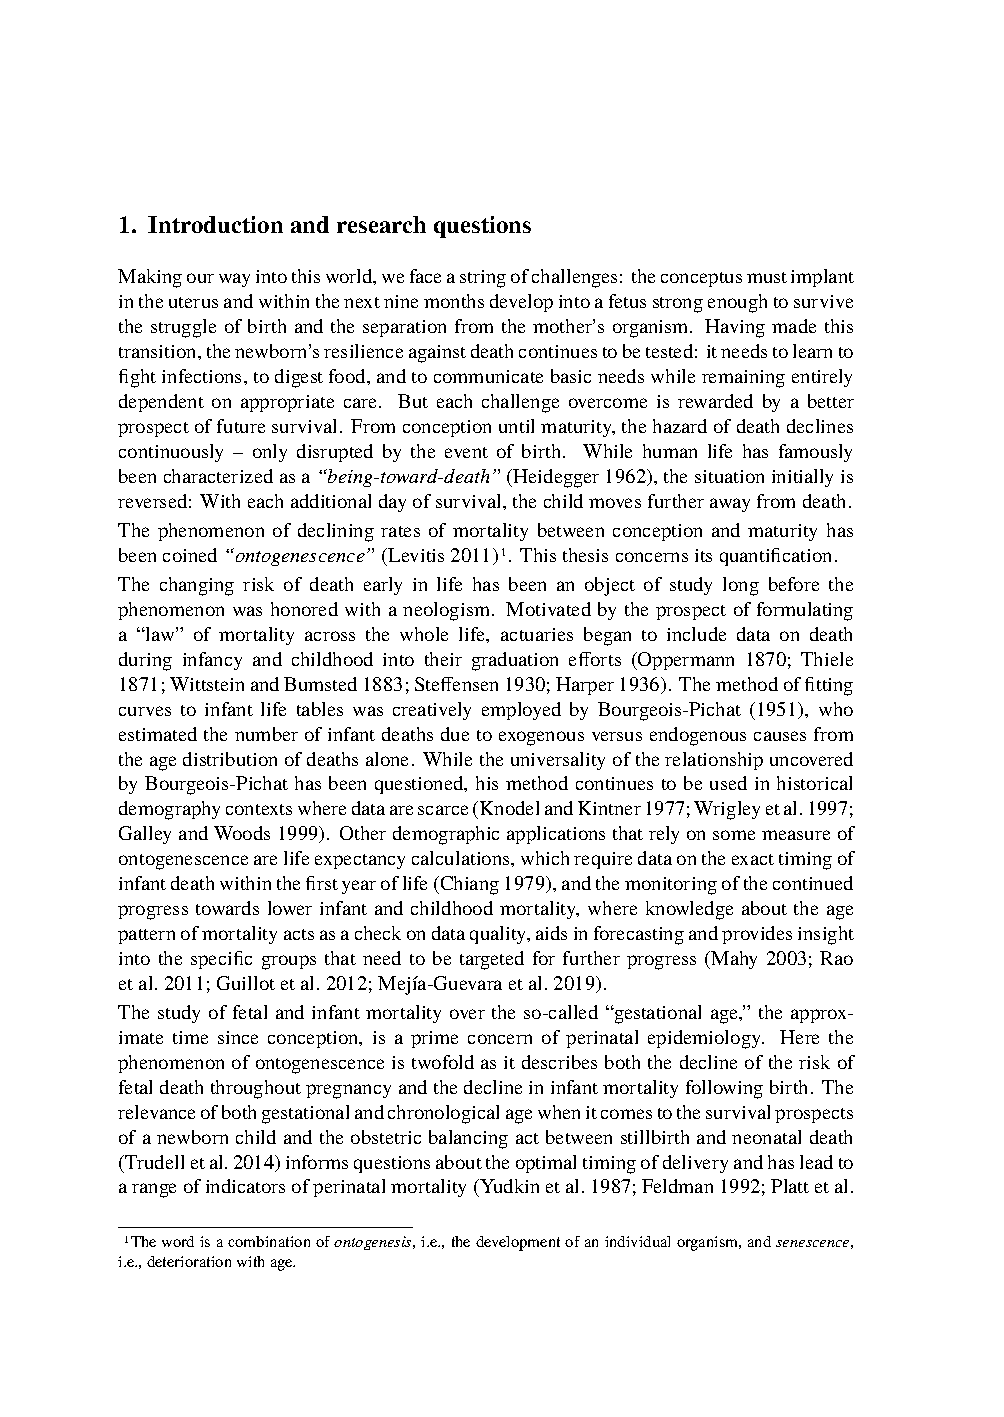
\includepdf[pages=-,pagecommand={\thispagestyle{headings}}]{./10-introduction/introduction.pdf}

\chapter{A parametric family of hazard trajectories for infant mortality}
\chaptermark{A parametric family}

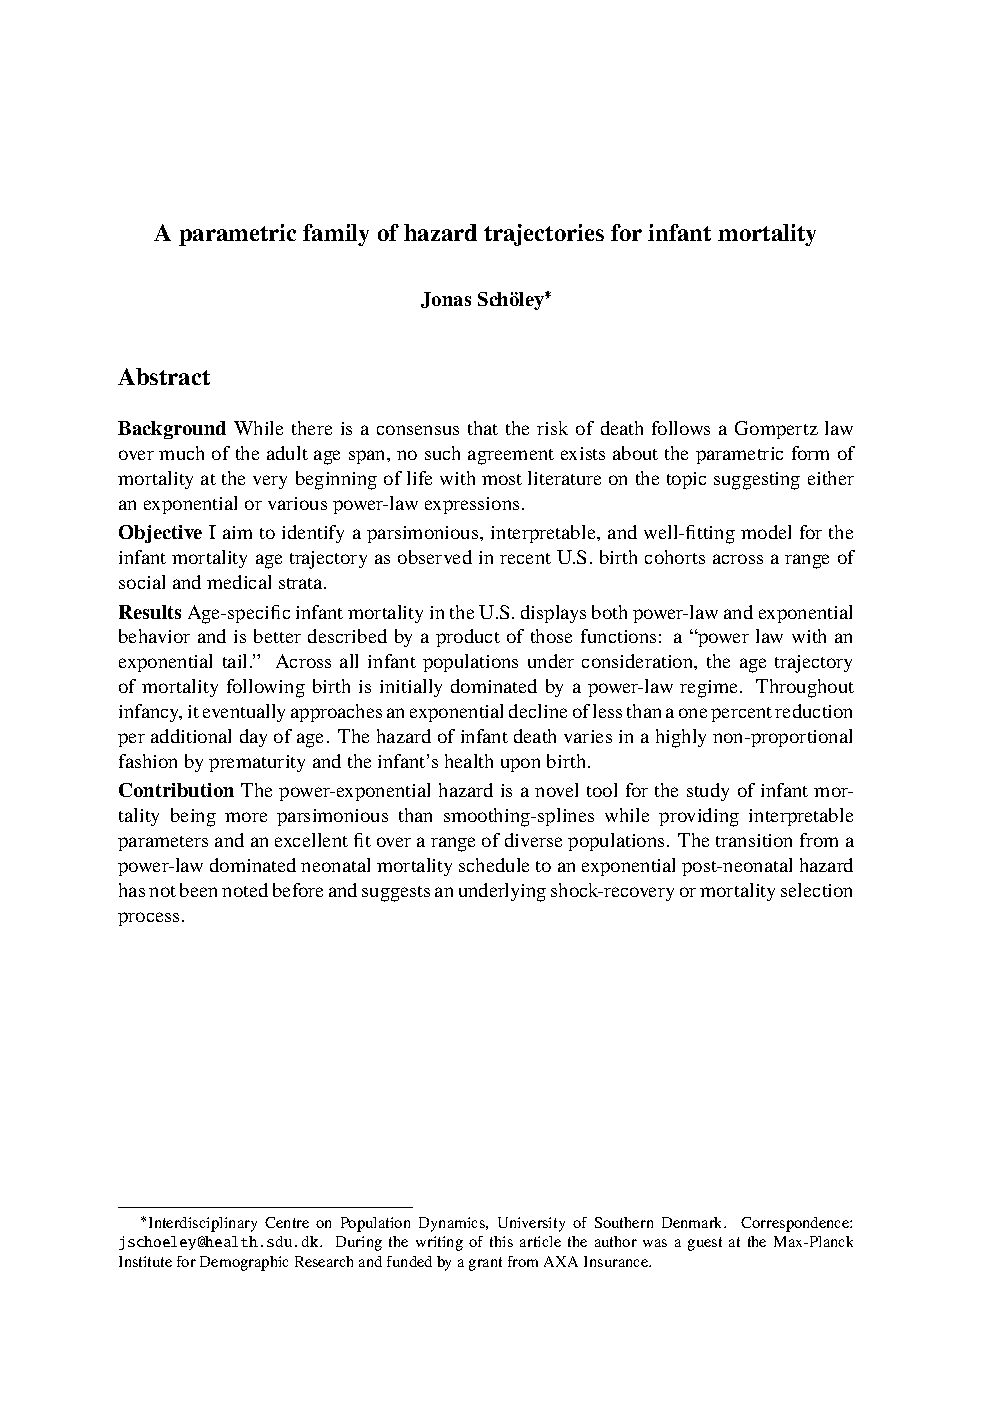
\includepdf[pages=-,pagecommand={\thispagestyle{headings}}]{./11-parametric_models_of_infant_mortality/parametric_models_of_infant_mortality.pdf}

\chapter{The impact of population heterogeneity on the age trajectory of neonatal mortality}
\chaptermark{The impact of population heterogeneity}

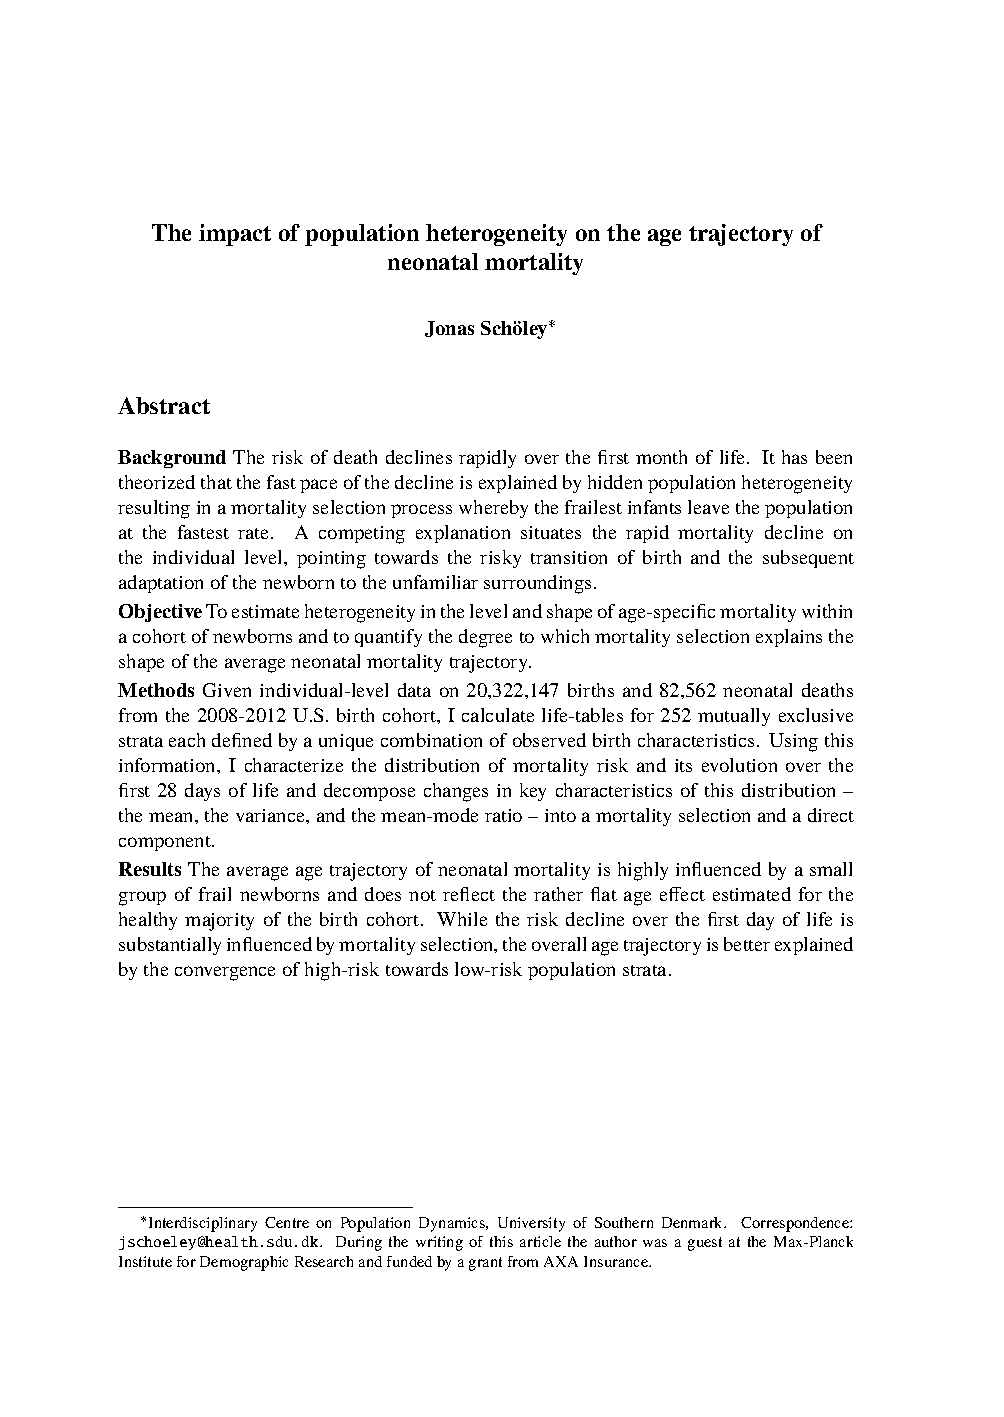
\includepdf[pages=-,pagecommand={\thispagestyle{headings}}]{./12-the_impact_of_mortality_selection/the_impact_of_mortality_selection.pdf}

\chapter{The gestational age pattern of feto-infant mortality}
\chaptermark{The gestational age pattern}

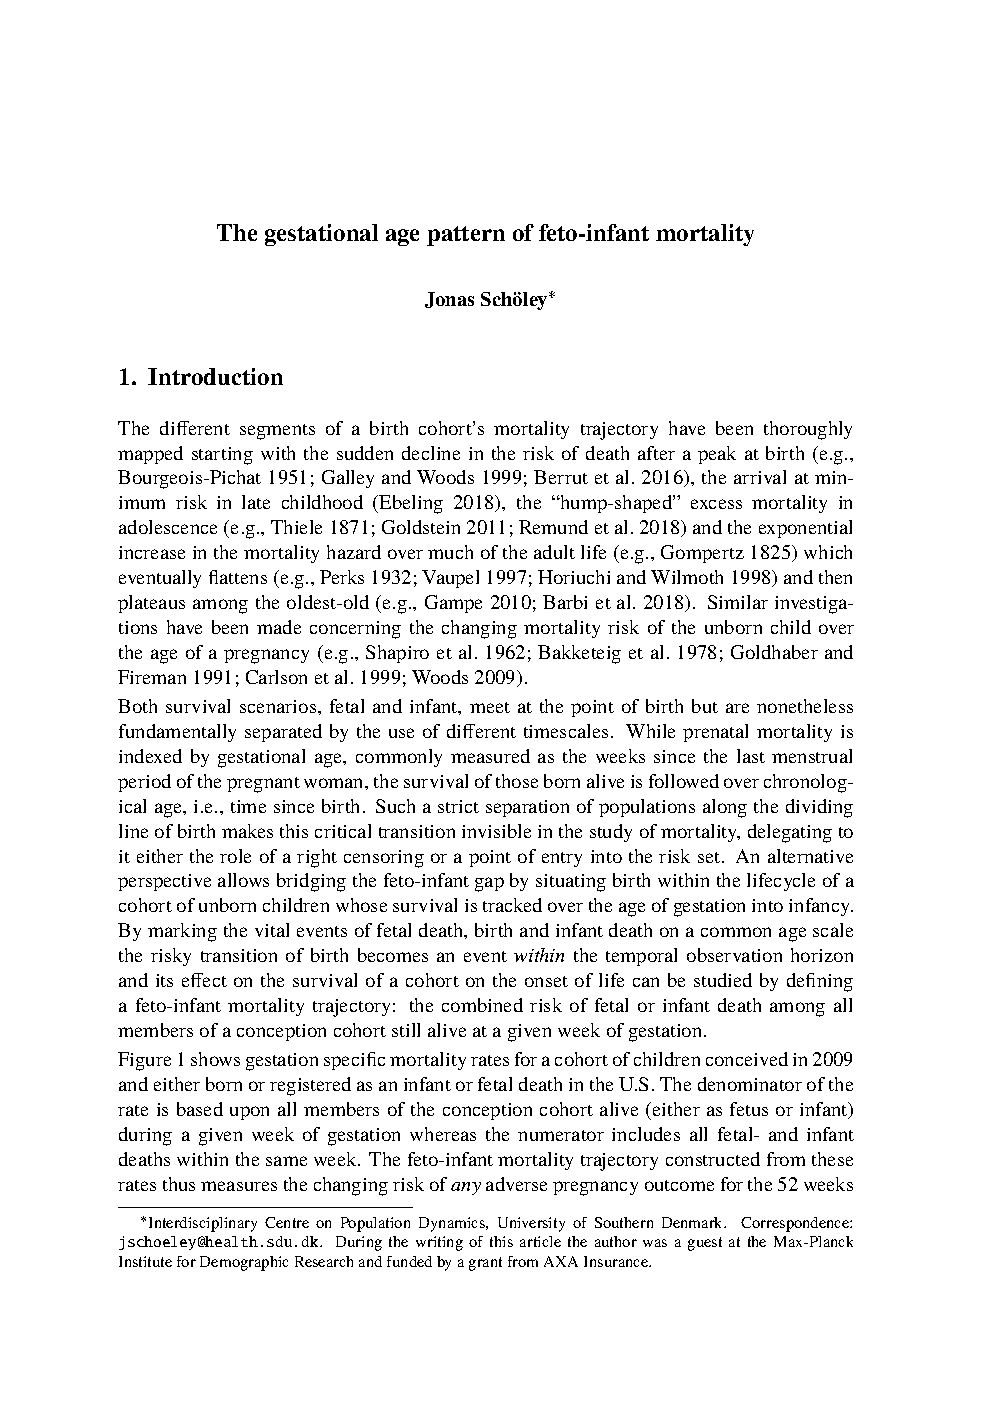
\includepdf[pages=-,pagecommand={\thispagestyle{headings}}]{./13-the_gestational_age_pattern/the_gestational_age_pattern.pdf}

\end{document}